\documentclass{beamer}
\usepackage{ctex}
\usetheme{SimplePlus}
\setbeamertemplate{footline}{}

\usepackage{amsmath,amssymb,mathtools}
\usepackage{tikz}
\usetikzlibrary{arrows.meta}
\usepackage{tikz-cd}

\usepackage{unicode-math}
%\setmathfont{STIX Two Math}
%\setmathfont{TeX Gyre Termes Math}
%\setmathfont{Libertinus Math}
%\setmathfont{Fira Math}

\usepackage[
  hybrid,                            % 允许在 Markdown 中混用 LaTeX 命令
  texMathDollars                     % 启用 $...$ 和 $$...$$ 数学公式
]{markdown}

\usepackage{graphicx} % Allows including images
\graphicspath{{./images/}}

\title{Kan}

\date{}

\begin{document}

\begin{frame}
    % Print the title page as the first slide
    \titlepage
\end{frame}

\begin{frame}[fragile]{Kan extension motivation}
The \emph{Kan extension} of a functor $F \colon \mathcal{C} \to \mathcal{D}$ with respect to a functor
\[
\begin{tikzcd}
\mathcal{C} \arrow[d, "p"] \\
\mathcal{C}'
\end{tikzcd}
\]
is, if it exists, a kind of \emph{best approximation} to the problem of finding a functor $\mathcal{C}' \to \mathcal{D}$ such that
\[
\begin{tikzcd}
\mathcal{C} \arrow[r, "F"] \arrow[d, "p"'] & \mathcal{D} \\
\mathcal{C}' \arrow[ur]
\end{tikzcd}
\]
hence to \emph{extending} the \emph{domain} of $F$ through $p$ from $\mathcal{C}$ to $\mathcal{C}'$.
\end{frame}

\begin{frame}[fragile]{Kan lift motivation}
Similarly, a \emph{Kan lift} is the best approximation to lifting a morphism $F \colon \mathcal{C} \to \mathcal{D}$ through a morphism
\[
\begin{tikzcd}
\mathcal{D}' \arrow[d] \\
\mathcal{D}
\end{tikzcd}
\]
to a morphism $\hat{F}$
\[
\begin{tikzcd}
 & \mathcal{D}' \arrow[d] \\
\mathcal{C} \arrow[r, "F"] \arrow[ur, "\hat{F}"] & \mathcal{D}.
\end{tikzcd}
\]
\end{frame}

\begin{frame}[fragile,shrink]{\cite{blog_kan}}
If you think of functor composition as a form of multiplication, Kan extensions
are an attempt to construct inverses of this multiplication. But unlike
multiplication, composition is not symmetric, so we have \emph{extensions} that
attempt to undo precomposition, and \emph{lifts} that do the same for
postcomposition. Furthermore, there rarely is a single inverse to any form of
composition, so we have the parsimonious \emph{right} extensions and lifts, and
the generous \emph{left} extensions and lifts. We end up with four combinations
that correspond to four different adjunctions:
\begin{align*}
(- \circ j) &\dashv \operatorname{Ran}_j - \\
\operatorname{Lan}_j - &\dashv (- \circ j) \\
(j \circ -) &\dashv \operatorname{Rift}_j - \\
\operatorname{Lift}_j - &\dashv (j \circ -)
\end{align*}
We'll concentrate on the extensions, since we can provide explicit point-wise
formulas for them in cases that are of interest to us, that is in $\mathbf{Cat}$
and in $\mathbf{Prof}$.
\end{frame}

\begin{frame}[fragile,shrink]
不要把
$$
\operatorname{Lan}_j
$$

或者
$$
\operatorname{Ran}_j
$$

理解成真正的 inverse。

通常：
$$
\operatorname{Lan}_j(G)\circ j
\not=
G
$$

甚至：
$$
\operatorname{Ran}_j(G)\circ j
\not=
G.
$$

它们只是分别通过：
$$
G\Rightarrow(\operatorname{Lan}_jG)\circ j
$$

和
$$
(\operatorname{Ran}_jG)\circ j\Rightarrow G
$$

给出一种 \textbf{universal approximation}。

所以作者所谓：
$$
\boxed{
\text{generous vs. parsimonious}
}
$$

真正应该理解成：
$$
\boxed{
\begin{array}{c}
\text{Left Kan extension}\\
\text{initial universal solution}\\
\text{自由、尽可能扩张}\\
\Downarrow\\
\text{generous}
\end{array}
\qquad
\begin{array}{c}
\text{Right Kan extension}\\
\text{terminal universal solution}\\
\text{保守、尽可能约束}\\
\Downarrow\\
\text{parsimonious}
\end{array}
}
$$

而这个直觉又恰好与：
$$
\boxed{
\operatorname{Lan}\sim\operatorname{colimit}
\qquad
\operatorname{Ran}\sim\operatorname{limit}
}
$$

相吻合。
\end{frame}

\begin{frame}[fragile]{left Kan extension}
A left Kan extension of a functor $F\colon\mathcal{C}\to\mathcal{E}$ along $K\colon\mathcal{C}\to\mathcal{D}$ consists of a functor $\operatorname{Lan}_K F\colon\mathcal{D}\to\mathcal{E}$ and a unit natural transformation $\eta\colon F\Rightarrow\operatorname{Lan}_K F\circ K$ such that for any other extension pair $(G\colon\mathcal{D}\to\mathcal{E},\gamma\colon F\Rightarrow G\circ K)$, there is a unique $\mu\colon\operatorname{Lan}_K F\Rightarrow G$ yielding the factorization $\gamma=\mu K\circ\eta$. This can be visualized by the pasting diagram
\begin{center}
  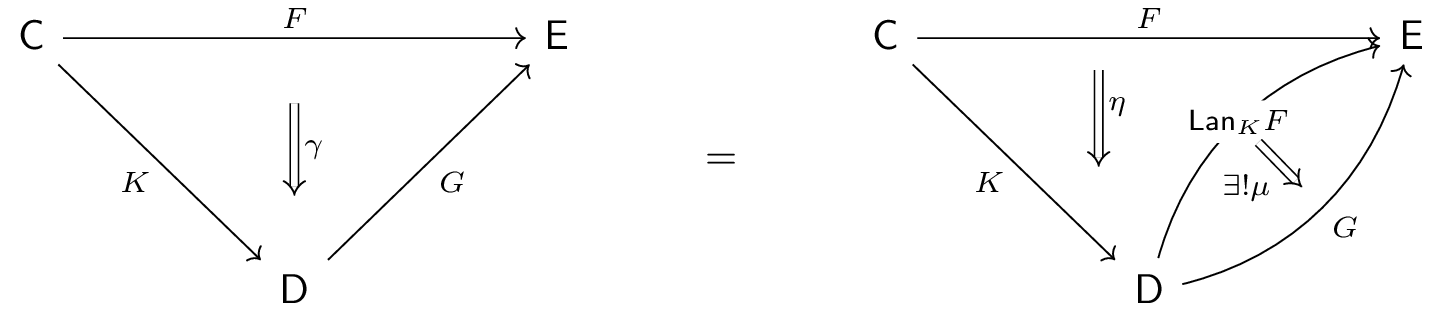
\includegraphics[width=\linewidth]{left-kan-univ}
\end{center}
\end{frame}

\begin{frame}[fragile]{right Kan Extension}
What's left is what's on the right, and indeed there is a dual notion of a right Kan extension, consisting of a functor $\operatorname{Ran}_K F\colon\mathcal{D}\to\mathcal{E}$ and counit natural transformation $\varepsilon\colon\operatorname{Ran}_K F\circ K\Rightarrow F$ such that for any other extension pair $(G\colon\mathcal{D}\to\mathcal{E},\delta\colon G\circ K\Rightarrow F)$, there is a unique $\mu\colon G\Rightarrow\operatorname{Ran}_K F$ yielding the factorization $\delta=\varepsilon\circ\mu K$.
\begin{center}
  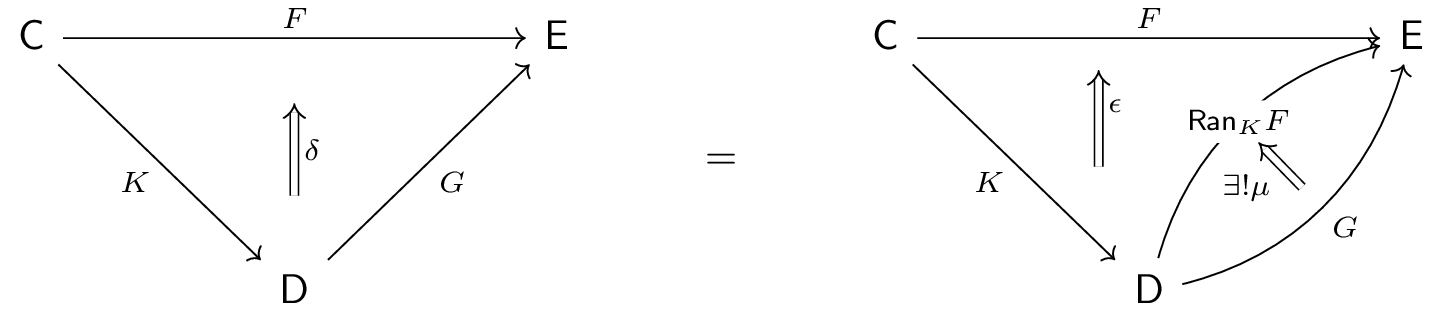
\includegraphics[width=\linewidth]{right-kan-univ}
\end{center}
\end{frame}

\begin{frame}{Building Kan Extensions}
We have already discussed the notion that Kan extensions are a kind-of approximation for a true extension, modulo a natural transformation. In particular, a left Kan extension of $F\colon\mathcal{C}\to\mathcal{E}$ along $K\colon\mathcal{C}\to\mathcal{D}$ is the ``best'' approximation of an extension of $F$ along $K$ ``from the left'', which is to say up to a natural transformation $\eta\colon F\Rightarrow\operatorname{Lan}_K F\circ K$ initial among all natural transformations $F\Rightarrow GK$ via an arrow $\operatorname{Lan}_K F\Rightarrow G$ ``from the left''. Taking this idea of ``approximating from the left'' to heart, to define the action of $\operatorname{Lan}_K F$ on an object $d$ we may want to consider the action of $F$ on objects in $\mathcal{C}$ that ``approximate'' $d$.
\end{frame}
\begin{frame}
In the present context, there are two reasonable ways to determine what objects ``approximate'' $d$. One is to choose those objects $c\in\mathcal{C}$ such that $Kc\cong d$. Another is to choose objects $c\in\mathcal{C}$ whose image under $K$ can ``get to'' $d$, which is to say there is an arrow $Kc\to d$. Indeed, considering the idea of approximation most universally, the latter feels more appropriate. Such ``approximating'' arrows $Kc\to d$ are exactly the objects of the comma category $K\downarrow d$, which has a canonical projection functor $\Pi^d\colon K\downarrow d\to\mathcal{C}$ that takes an arrow $Kc\to d$ defining an ``approximation of $d$ from the left'' to the ``approximating object'' $c$. We can then map each such object via $F$, defining a diagram $K\downarrow d\xrightarrow{\Pi^d}\mathcal{C}\xrightarrow{F}\mathcal{E}$ whose image seemingly provides a number of approximations for the image of $d$ ``from the left''. How do we collapse these approximations into a single object? Take a colimit!
\end{frame}

\begin{frame}[fragile]
\textbf{Theorem.} Consider $F\colon\mathcal{C}\to\mathcal{E}$ and $K\colon\mathcal{C}\to\mathcal{D}$. If $\forall d\in\mathcal{D}$ the colimit
\[
\operatorname{colim}\bigl(K\downarrow d\xrightarrow{\Pi^d}\mathcal{C}\xrightarrow{F}\mathcal{E}\bigr)=:\operatorname{Lan}_K F(d)
\]
of the diagram $F\Pi^d$ exists, these data assemble into a functor $\operatorname{Lan}_K F\colon\mathcal{D}\to\mathcal{E}$, and the colimit cones embed the unit $\eta\colon F\Rightarrow\operatorname{Lan}_K F\circ K$, such that $\operatorname{Lan}_K F,\eta$ define the left Kan extension of $F$ along $K$.

Dually, if $\forall d\in\mathcal{D}$ the limit
\[
\lim\bigl(d\downarrow K\xrightarrow{\Pi_d}\mathcal{C}\xrightarrow{F}\mathcal{E}\bigr)=:\operatorname{Ran}_K F(d)
\]
of the diagram $F\Pi_d$ exists, these data assemble into a functor $\operatorname{Ran}_K F\colon\mathcal{D}\to\mathcal{E}$, and the limit cones embed the counit $\varepsilon\colon\operatorname{Ran}_K F\circ K\Rightarrow F$, such that $\operatorname{Ran}_K F,\varepsilon$ define the right Kan extension of $F$ along $K$.
\end{frame}

\begin{frame}[fragile]{}
\textbf{Adjunction：}
$$
F\dashv G
$$

可以特殊地编码为：
$$
G=\operatorname{Lan}_F1,
$$

或者：
$$
F=\operatorname{Ran}_G1.
$$

\textbf{Limit / colimit：}

又是 Kan extension 的另一个特殊情形：
$$
\boxed{
\operatorname{colim}F
=
\operatorname{Lan}_{!}F
}
$$

$$
\boxed{
\operatorname{lim}F
=
\operatorname{Ran}_{!}F
}
$$

其中：
$$
!:\mathcal C\to\mathbf 1.
$$
\end{frame}

% 参考文献帧，长列表自动分页
\begin{frame}[allowframebreaks]{参考文献}
\begin{thebibliography}{99}

\bibitem{ncatlab_kan}
\url{https://ncatlab.org/nlab/show/Kan+extension}

\bibitem{blog_kan}
\url{https://bartoszmilewski.com/2026/06/08/kan-extensions-in-haskell/}

\bibitem{fly_kan}
\url{https://ayazhafiz.com/articles/21/a-flying-tour-of-kan-extensions}

\end{thebibliography}
\end{frame}
\end{document}